% =====================================================================
% THIS FILE IS THE SOURCE. Edit it, then rebuild the PDF with:
%     bash tools/compile.sh Unit_02_Probability_and_Random_Variables
% (run from the Course_Rewrite folder; it compiles twice and reports
%  page count, overfull boxes, and em dashes)
%
% Do not edit the PDF directly. Figures are the fig_*.pdf files in this
% folder, regenerated by tools/make_module*_slide_figs.py.
%
% Originally converted from the 15-module draft by a one-shot script now
% parked in tools/one_shot_generators/. Re-running those would discard
% anything you change here, so they are kept out of tools/ on purpose.
% =====================================================================
\documentclass[aspectratio=169]{beamer}
\usetheme{default}
\usefonttheme{professionalfonts}
\usepackage{amsmath, amssymb, amsfonts}
\usepackage{graphicx}
\usepackage{booktabs}
\usepackage{bm}
\usepackage{hyperref}

\mode<presentation> {
    \usetheme{Frankfurt}
    \usecolortheme{default}
}

% == notation shortcuts ==
\newcommand{\xbar}{\bar{x}}
\newcommand{\PR}[1]{P(#1)}
\newcommand{\E}[1]{E[#1]}
\newcommand{\Var}[1]{\mathrm{Var}(#1)}
\newcommand{\SD}[1]{\mathrm{SD}(#1)}

% Recurring motifs (color-coded).
\newenvironment{principle}[1]{\begin{block}{\textbf{Principle:} #1}}{\end{block}}
\newenvironment{trap}[1]{\begin{alertblock}{\textbf{Trap:} #1}}{\end{alertblock}}
\newenvironment{practice}[1]{\begin{exampleblock}{\textbf{In practice:} #1}}{\end{exampleblock}}
\newenvironment{interview}[1]{\begin{exampleblock}{\textbf{You may be asked:} #1}}{\end{exampleblock}}
\newenvironment{yourturn}[1]{%
  \setbeamercolor{block title}{fg=white,bg=orange!80!black}%
  \setbeamercolor{block body}{bg=orange!12}%
  \begin{block}{\textbf{Your turn:} #1}}{\end{block}}
\newenvironment{livedemo}[1]{%
  \setbeamercolor{block title}{fg=white,bg=teal!80!black}%
  \setbeamercolor{block body}{bg=teal!12}%
  \begin{block}{\textbf{Live demo:} #1}}{\end{block}}
\newenvironment{llmcheck}[1]{%
  \setbeamercolor{block title}{fg=white,bg=violet!75!black}%
  \setbeamercolor{block body}{bg=violet!10}%
  \begin{block}{\textbf{LLM check:} #1}}{\end{block}}

\title{Random Variables and Distributions}
\subtitle{Unit 8: Putting a Number on an Uncertain Thing}
\author{Stat 220 \textbar{} Statistics for Data Science}
\date{}

\begin{document}

\begin{frame}
  \titlepage
\end{frame}

% ======================================================================
\section{Random variables}
% ======================================================================
\begin{frame}{Where this fits}
\begin{itemize}
  \item Unit 7 dealt in events: did the customer buy, is the test positive, did the server fail.
  \item Now we attach a \textbf{number} to the outcome. Revenue, wait time, defects, dollars lost.
  \item Once outcomes are numbers we can average them, add them up, and compare decisions, which
        is where this becomes useful to somebody with a budget.
\end{itemize}
\begin{principle}{a random variable is a rule, not a value}
It is not ``the number that came up.'' It is the whole recipe: which numbers are possible and how
often each one occurs.
\end{principle}
\end{frame}

\begin{frame}{Live experiment: what will you pay to play?}
\begin{livedemo}{a sealed-bid auction for three gambles}
On a slip of paper write the \textbf{most you would pay} to play each game. One number each, no
conferring.
\begin{enumerate}
  \item \textbf{Game A:} I roll a die. You win \$60 if it shows a 6, otherwise nothing.
  \item \textbf{Game B:} I flip a coin. Heads you win \$20, tails nothing.
  \item \textbf{Game C:} I flip a coin. Heads you win \$2{,}000, tails you \emph{lose} \$1{,}000.
\end{enumerate}
\end{livedemo}
\vspace{0.2em}
{\tiny\textit{Materials: slips of paper. Time: 8 minutes. Do not reveal the expected values until the bids are collected.}}
\centering\small Pass them forward. We will find the highest bidder for each and compare the bids
to what the games are worth.
\end{frame}

\begin{frame}{Stay here while they bid: what each game is worth}
\begin{itemize}
  \item Game A: $\tfrac{1}{6}(60) + \tfrac{5}{6}(0) = \$10$.
  \item Game B: $\tfrac{1}{2}(20) + \tfrac{1}{2}(0) = \$10$.
  \item Game C: $\tfrac{1}{2}(2000) + \tfrac{1}{2}(-1000) = \$500$.
\end{itemize}
\onslide<2->{
Two predictions about your slips:
\begin{itemize}
  \item A and B are worth the same, but B usually draws higher bids. The \emph{spread} bothers
        you, not just the average.
  \item Almost nobody bids near \$500 for C, even though it is worth fifty times the others.
\end{itemize}
That instinct is correct, and it is why this day covers \textbf{two} numbers, not one.}
\end{frame}

\begin{frame}{What this unit gives you}
\begin{columns}[T]
\begin{column}{0.5\textwidth}
\textbf{Things to know}
\begin{itemize}\small
  \item expectation as a long-run average, and its linearity
  \item variance and standard deviation, in the right units
  \item what happens to the mean and spread when you add things up
  \item which standard distribution matches which real-world story
  \item why plugging an average into a curved calculation is wrong
\end{itemize}
\end{column}
\begin{column}{0.5\textwidth}
\textbf{Mistakes to stop making}
\begin{itemize}\small
  \item reporting a mean with no measure of spread
  \item treating the mean as typical when the data is skewed
  \item computing the answer at average inputs instead of averaging the answers
  \item adding variances of things that are not independent
  \item picking a distribution by eyeballing a histogram
\end{itemize}
\end{column}
\end{columns}
\end{frame}

\begin{frame}{Random variables and expectation}
A \textbf{random variable} is not ``the number that came up.'' It is the whole recipe: which
numbers are possible and how often each occurs.
\[
\E{X} \;=\; \sum_x x \cdot \PR{X = x}
\]
\begin{itemize}
  \item The expectation is the average you would see over a very large number of repetitions.
  \item It need not be a possible value: the expected number of children per family is 2.3, and no
        family has 2.3 children.
\end{itemize}
\begin{principle}{expectation answers ``in the long run,'' not ``this time''}
It is the right tool for decisions you make repeatedly, and a dangerous one for a decision you
make once with everything on the line.
\end{principle}
\end{frame}

\begin{frame}{Linearity: the most useful fact in this course}
For \emph{any} random variables, independent or not:
\[
\E{aX + b} = a\E{X} + b, \qquad \E{X + Y} = \E{X} + \E{Y}.
\]
\begin{itemize}
  \item No independence required. That is why expectations are so pleasant to work with.
  \item \textbf{Worked example.} A call center takes 400 calls a day. Each caller buys with
        probability 0.06, spending \$85. Write $R = \sum_{i=1}^{400} 85\, I_i$ where $I_i$ is 1 if
        caller $i$ buys. Then $\E{R} = 400 \times 85 \times 0.06 = \$2{,}040$.
  \item We never needed the distribution of daily revenue. Linearity gave us the mean without
        it.
\end{itemize}
\end{frame}

\begin{frame}{Variance: how far things swing}
\[
\Var{X} = \E{(X - \E{X})^2}, \qquad \SD{X} = \sqrt{\Var{X}}.
\]
\begin{itemize}
  \item Variance is in squared units (dollars squared), which nobody can interpret. Report the
        \textbf{standard deviation}, which is in the original units.
  \item $\Var{aX + b} = a^2 \Var{X}$: shifting does nothing, scaling squares.
  \item For \textbf{independent} $X$ and $Y$: $\Var{X + Y} = \Var{X} + \Var{Y}$. Variances add, so
        standard deviations grow like $\sqrt{n}$, not $n$.
\end{itemize}
\begin{trap}{the independence clause, again}
``Variances add'' is not a law of nature. It is a reward for independence, and it is the same
assumption that failed in 2008.
\end{trap}
\end{frame}

\begin{frame}{Why averaging works, and when it stops}
\begin{columns}[c]
\begin{column}{0.58\textwidth}
\centering
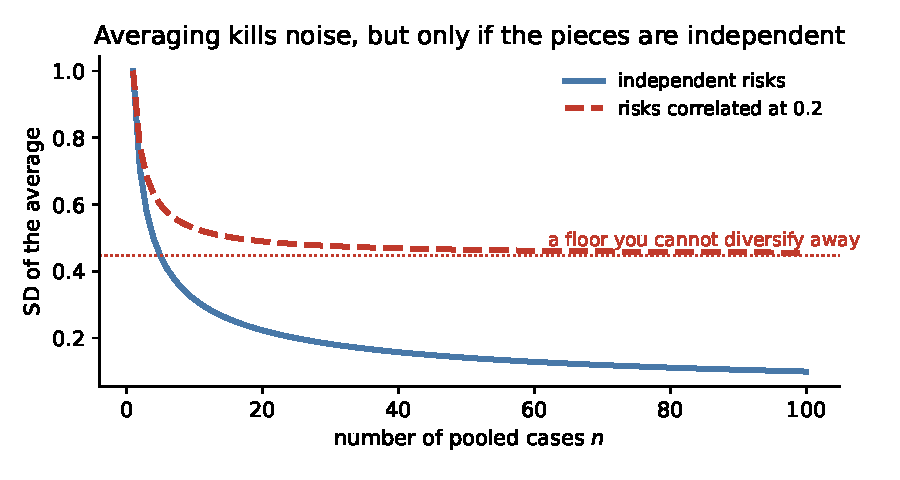
\includegraphics[width=\textwidth]{fig_m06_pooling.pdf}
\end{column}
\begin{column}{0.42\textwidth}
\small
The SD of an average of $n$ independent cases falls like $1/\sqrt{n}$.
\begin{itemize}
  \item Four times the data, half the noise. That is the entire economics of sample size, and you
        met it in Unit 1 as $\sigma/\sqrt{n}$.
  \item If the cases are correlated, the curve flattens onto a floor you cannot buy your way
        below.
\end{itemize}
\end{column}
\end{columns}
\onslide<2->{\centering\small
This one picture is insurance, portfolio diversification, and A/B testing, and also why a pandemic
or a market crash breaks all three at once.}
\end{frame}

\begin{frame}{Your turn \#1}
\begin{yourturn}{same average, different animal}
Two ad campaigns each have an expected return of \$50{,}000.
\begin{itemize}
  \item Campaign A returns somewhere between \$40k and \$60k.
  \item Campaign B has a 90\% chance of \$0 and a 10\% chance of \$500k.
\end{itemize}
With a neighbor: which do you recommend, and what do you need to know about the company first?
\end{yourturn}
\end{frame}

\begin{frame}{Your turn \#1: answer}
\begin{itemize}
  \item There is no answer without context. The real questions are \textbf{how many times you get
        to play} and \textbf{what a zero costs you}.
  \item A firm running 50 campaigns a year should take B. The averaging in the last picture turns
        its variance into a reliable return.
  \item A startup that must make payroll next month should take A. One draw of \$0 ends the
        company, and there is no long run for a company that no longer exists.
\end{itemize}
\begin{principle}{expected value assumes you survive to repeat}
Maximize expected value across many bets you can absorb. For a single bet you cannot recover from,
look at the downside instead.
\end{principle}
\end{frame}

\begin{frame}{Pick the distribution by the mechanism}
\begin{columns}[c]
\begin{column}{0.6\textwidth}
\centering
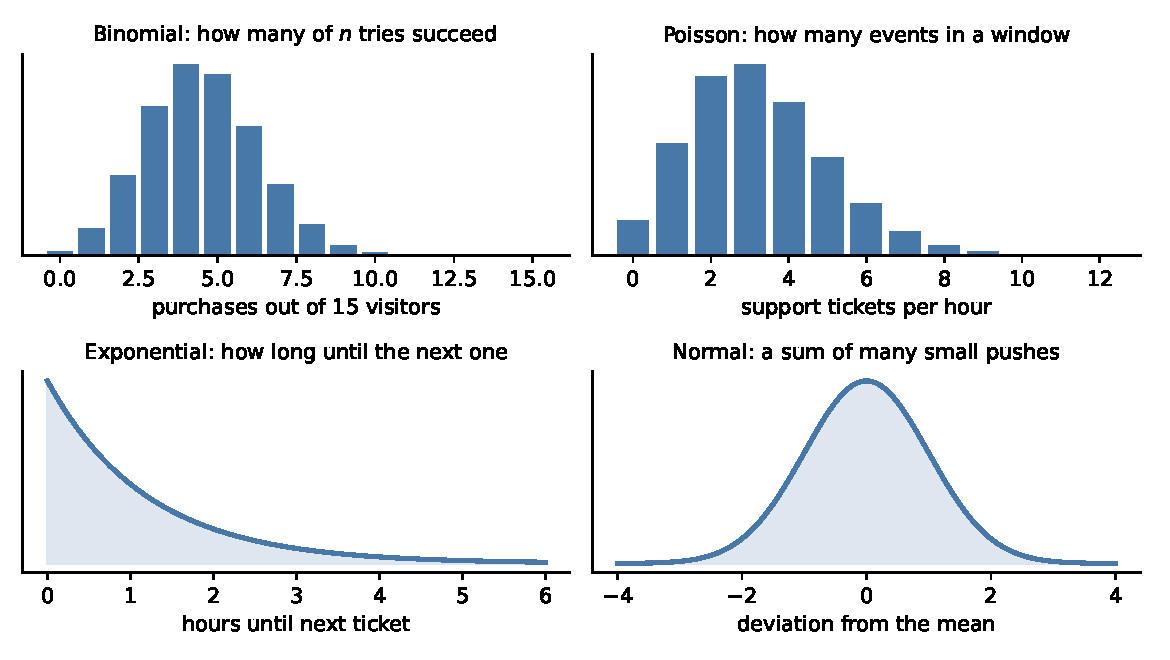
\includegraphics[width=\textwidth]{fig_m06_dists.pdf}
\end{column}
\begin{column}{0.4\textwidth}
\small
Each shape comes from a \emph{story} about how the data is generated. Learn the four stories and
the formulas follow.
\end{column}
\end{columns}
\end{frame}

\begin{frame}{The four stories worth memorizing}
\begin{itemize}
  \item \textbf{Bernoulli / Binomial:} a fixed number of independent yes-or-no tries, each with
        the same chance. ``How many of 500 visitors converted?'' $\E{X} = np$,
        $\Var{X} = np(1-p)$.
  \item \textbf{Poisson:} events arriving at a steady rate in a window of time or space. ``How
        many tickets this hour?'' Mean and variance are both $\lambda$.
  \item \textbf{Exponential:} the waiting time \emph{until} the next such event.
  \item \textbf{Normal:} anything built from many small independent contributions added together.
        Unit 3 is entirely about why this one shows up everywhere.
\end{itemize}
\end{frame}

\begin{frame}{Choosing a model in practice}
\begin{itemize}
  \item Ask what generated the number, not what the histogram looks like.
  \item Counts of successes out of a known number of tries: binomial. Counts with no natural
        ceiling, arriving over time: Poisson.
  \item Waiting times, durations, and time-to-failure: exponential-ish, and almost always
        right-skewed.
  \item Money is almost never normal. Revenue per customer, income, and claim sizes are skewed
        with a long right tail.
\end{itemize}
\begin{trap}{a check worth running}
Poisson forces the variance to equal the mean. Real count data is usually \emph{over}-dispersed,
with variance well above the mean, because the underlying rate itself varies (Mondays, launches,
outages). Check that before trusting a Poisson.
\end{trap}
\end{frame}

\begin{frame}{Averages plugged into nonlinear things}
\begin{columns}[c]
\begin{column}{0.58\textwidth}
\centering
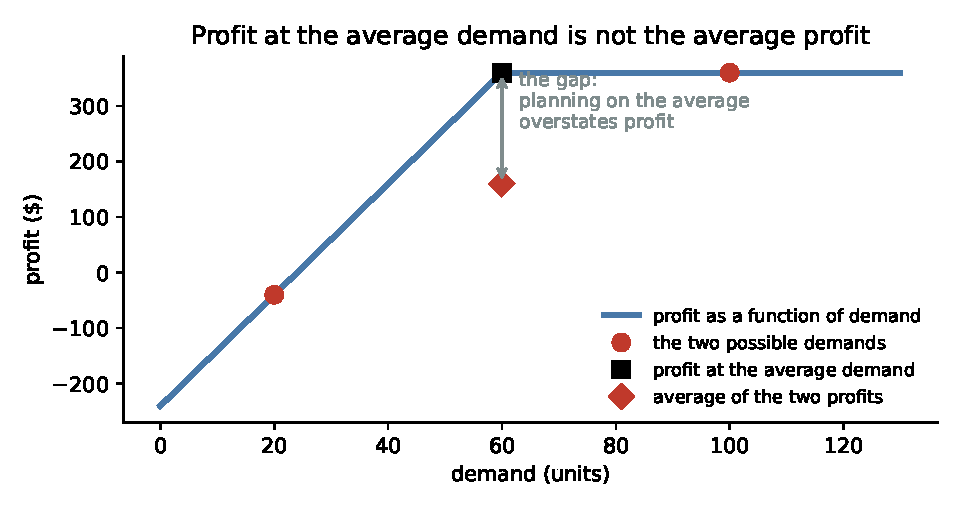
\includegraphics[width=\textwidth]{fig_m06_flaw.pdf}
\end{column}
\begin{column}{0.42\textwidth}
\small
Capacity is 60 units, each sold for \$10, each unit of capacity costs \$4. Demand is 20 or 100,
equally likely.
\begin{itemize}
  \item Profit at the \emph{average} demand of 60: \textbf{\$360}.
  \item \emph{Average} profit across the two demands: \textbf{\$160}.
\end{itemize}
The plan built on the average overstates profit by more than double.
\end{column}
\end{columns}
\end{frame}

\begin{frame}{Why the gap appears}
\begin{itemize}
  \item Whenever the quantity you care about is a \textbf{curved} function of an uncertain input,
        $\E{f(X)} \neq f(\E{X})$.
  \item Caps, floors, thresholds, penalties, stockouts, and SLA cliffs are all curves. Business is
        made of them.
  \item ``A statistician drowned crossing a river of average depth three feet.''
\end{itemize}
\begin{trap}{planning on the average}
Any plan built by replacing every uncertain input with its mean will be systematically wrong, and
usually optimistic, because it ignores the bad tail where the penalties live.
\end{trap}
\end{frame}

\begin{frame}{The mean is not the typical case}
\begin{columns}[c]
\begin{column}{0.58\textwidth}
\centering
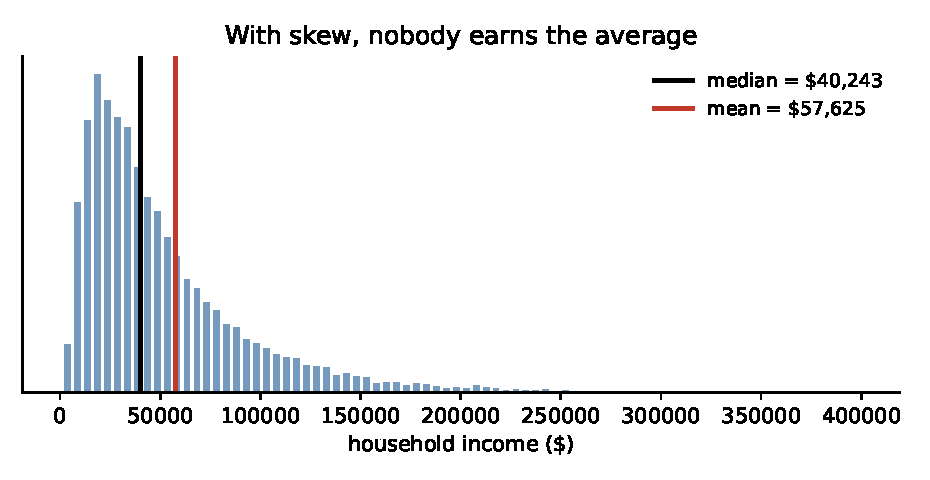
\includegraphics[width=\textwidth]{fig_m06_skew.pdf}
\end{column}
\begin{column}{0.42\textwidth}
\small
With right-skewed data the mean sits well above the median, dragged up by the tail.
\begin{itemize}
  \item ``Average revenue per user'' in a business where 2\% of users are whales describes nobody.
  \item Report the median, the mean, and something about the tail. They answer different
        questions.
\end{itemize}
\end{column}
\end{columns}
\onslide<2->{\centering\small
Rule of thumb: when the mean and median differ a lot, someone is about to be misled.}
\end{frame}

% ======================================================================
\section{Consolidate}
% ======================================================================
\begin{frame}{Modeling an uncertain quantity, in order}
\small
\begin{enumerate}
  \item \textbf{Define the variable in words and units.} ``Tickets per hour,'' not ``tickets.''
  \item \textbf{Tell the generating story.} Fixed tries? Arrivals over time? A waiting time? A sum
        of many small pieces?
  \item \textbf{Pick the distribution the story implies}, and write down what it assumes.
  \item \textbf{Get the mean and the SD}, and sanity-check both against reality.
  \item \textbf{Check the assumption that breaks first}, usually independence or a constant rate.
  \item \textbf{Compute the decision quantity by simulation}, never by plugging in averages.
\end{enumerate}
\end{frame}

\begin{frame}{What you should be able to do with software}
\small
Nobody is asking you to memorize syntax. You are expected to know \emph{which} procedure the
question calls for and what the output means.
\begin{center}\footnotesize
\begin{tabular}{p{0.44\textwidth} p{0.46\textwidth}}
\toprule
\textbf{You should be able to} & \textbf{What you would reach for} \\
\midrule
Mean and SD of a simulated quantity & \texttt{.mean()}, \texttt{.std(ddof=1)} \\
Exact binomial probabilities and tails & \texttt{stats.binom.pmf}, \texttt{.sf} \\
Counts over a window & \texttt{stats.poisson.pmf}, \texttt{.sf} \\
Waiting times & \texttt{stats.expon} \\
Check whether counts are over-dispersed & compare the sample variance to the mean \\
Expected profit or cost under uncertainty & simulate the scenarios, then average \\
Find the best decision, not the average one & sweep the choice and take the maximum \\
\bottomrule
\end{tabular}
\end{center}
\vspace{0.2em}
\centering\small
If you cannot say what the output means, producing it is worth nothing.
\end{frame}

\begin{frame}{The traps, all in one place}
\begin{trap}{the ones that bite most often}
\begin{itemize}
  \item Reporting a mean with no standard deviation or range.
  \item Calling the mean ``typical'' when the data is skewed.
  \item Computing the answer at average inputs instead of averaging the answers.
  \item Adding variances for things that share a driver.
  \item Choosing a distribution from a histogram instead of a mechanism.
  \item Maximizing expected value on a one-shot bet you cannot survive losing.
\end{itemize}
\end{trap}
\end{frame}

\begin{frame}{Ten questions to be able to answer}
\begin{enumerate}\small
  \item Define expected value and give a case where it is the wrong thing to maximize.
  \item Two projects have equal expected return. What else do you want to know?
  \item Why does the SD of an average shrink like $1/\sqrt{n}$, and when does it not?
  \item Our average customer spends \$80. What is wrong with planning around that?
  \item Why is profit at average demand not the same as average profit?
  \item Which distribution would you use for tickets per hour, and what does it assume?
  \item Your count data has variance three times its mean. What does that tell you?
  \item How would you staff when understaffing and overstaffing cost different amounts?
  \item Explain to a manager why the median and mean of our revenue differ.
  \item When would you simulate instead of using a formula?
\end{enumerate}
\end{frame}

\begin{frame}{Mastery checklist}
You have this unit when you can, from memory:
\begin{itemize}
  \item define a random variable, its expectation, and its standard deviation
  \item use linearity to break a total into pieces
  \item say what happens to the mean and SD when independent things are summed or averaged
  \item match binomial, Poisson, exponential, and normal to their generating stories
  \item explain the flaw of averages with a concrete example
  \item argue when expected value is and is not the right objective
\end{itemize}
\end{frame}

\begin{frame}{Where we go next}
\begin{itemize}
  \item We just saw that averages of many independent pieces get predictably tighter, like
        $1/\sqrt{n}$.
  \item \textbf{Unit 9} explains why, and shows they also take on a specific \emph{shape}. That
        result is what finally justifies every standard error you have used since Unit 1.
\end{itemize}
\begin{principle}{the habit to keep}
A number without a spread is a guess. The mean says where, the SD says how much to hedge.
\end{principle}
\end{frame}

\end{document}
